\documentclass{article}
\usepackage[utf8x]{inputenc} % codifica scrittura
\usepackage[nochapters]{classicthesis} % nochapters

%\usepackage{inputenc}
\usepackage[T1]{fontenc} 
\usepackage[square,numbers]{natbib} 
\usepackage{amsmath, amsthm, amssymb, tikz}
\usetikzlibrary{snakes}
% \newtheorem{definizione}{Definizione}  
% \newtheorem{lemma}{Lemma}
% \newtheorem{teorema}{Teorema}  
% \newtheorem{proprieta}{Proprietà}  
\usepackage{titletoc}
\usepackage{verbatim}
\usepackage{hyperref}

\titlecontents{section}[3em]{}{\contentslabel{1em}}{}{\titlerule*[1.5pc]{.}\contentspage}
\titlecontents{subsection}[6em]{}{\contentslabel{2em}}{}{\titlerule*[1.5pc]{.}\contentspage}

\begin{document}

\title{\rmfamily\normalfont\spacedallcaps{Computer Aided Graphic
    Design course exercises}}

\author{\spacedlowsmallcaps{Massimo Nocentini}}
\date{\today}

\maketitle


\begin{abstract}
  This document contains some exercises and collects work done during
  the CAGD course given by Prof. Alessandra Sestini and Prof. Costanza
  Conti at University of Florence.

  The content is organized in sections, each one of them correspond to
  a given set of exercises, the last one report the raw implementation
  code written in Julia \cite{Julia}.
\end{abstract}
       
\tableofcontents

\newpage

\section{Bezier curves}

\subsection{Curve from simple set of control points}
In \autoref{fig:first-closed-curve} we report the very first curve
obtained using our implementation reported in
\autoref{sec:deCasteljau-code}. The curve is obtained using control
points $(1,1), (3,4), (5,6),(7,8),(10,2),(1,1)$ in the given
order. This plot was the first test for our implementation of code
reported in Exercise 1 and requested in Exercise 2: it contains a
segmented curve in green which is the control polygon, and a Bezier
curve in red built using the given control points.
\begin{figure}
  \centering
  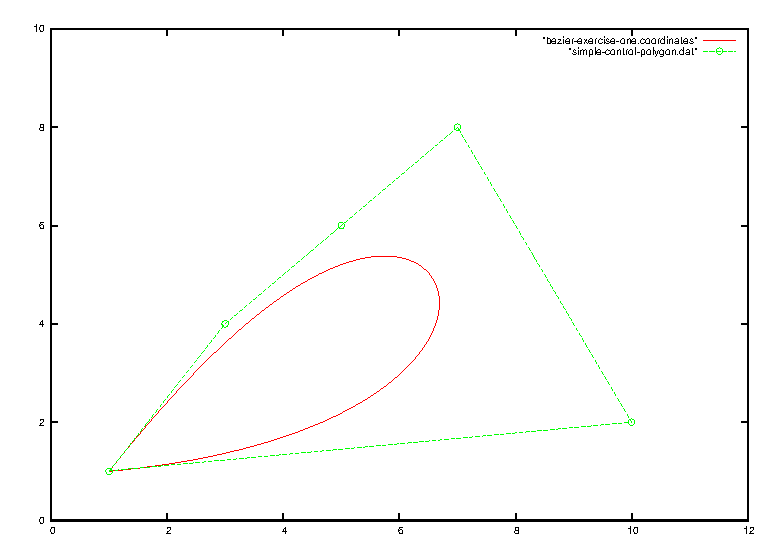
\includegraphics{bezier-deCasteljau-curves/exercise-one}  
  \caption{Curve from simple set of control points}
  \label{fig:first-closed-curve}
\end{figure}

\subsection{Curve from parametric specification}
As required in Exercise 3, in \autoref{fig:curve-from-parametric-spec}
we report a Bezier curve built from the parametric specification:
\begin{displaymath}
  \left [  \begin{array}{c}
      x(u) \\
      y(u)
    \end{array} \right ] = \left [  
    \begin{array}{c}
      1 + u + u^2 \\
      u^3
    \end{array} \right ]
\end{displaymath}
with $u\in[0,1]$. For plotting we choose to sample 6 control points,
uniformly spaced in $[0,1]$: observe that there isn't a relation
between the uniform sampling for the parameter $u$ and control points
distribution on the plane.
\begin{figure}
  \centering
  \includegraphics{bezier-deCasteljau-curves/exercise-two}
  \caption{Curve from parametric specification}
  \label{fig:curve-from-parametric-spec}
\end{figure}

\subsection{Splitted curve on a given parameter $u$}
As required in Exercise 4, in \autoref{fig:splitted-curve} we report
the control polygon, in red, for the original curve and two sets of
control points with the same cardinality that, drawn together, build a
Bezier that is the same as the original one. Those two sets are
colored in green (the relative Bezier in magenta) and in blue (the
relative Bezier in cyan), respectively.
\begin{figure}
  \centering
  \includegraphics{bezier-deCasteljau-curves/exercise-four}
  \caption{Splitted curve}
  \label{fig:splitted-curve}
\end{figure}

\subsection{Repeating the same control point more times}
As required in Exercise 5, in
\autoref{fig:repeating-same-control-point} we report two Bezier: the
red one relative to control points $\{(2,4), (6,12), (10,1),
(12,12)\}$ the green one relative to control points $\{(2,4), (6,12),
(10,1), (10,1), (10,1), (10,1), (12,12)\}$, ie. with the point
$(10,1)$ repeated three more times. We see that the Bezier relative to
the augmented control polygon goes down toward $(10,1)$ more than the
other Bezier: this can be explained from a probabilistic point of
view, since a Bezier can be thought as a \emph{mean} of the control
polygon, hence putting weight in $(10,1)$ increase the control point's
weight.
\begin{figure}
  \centering
  \includegraphics{bezier-deCasteljau-curves/exercise-five}
  \caption{Repeating the control point $(10,1)$ three more times}
  \label{fig:repeating-same-control-point}
\end{figure}

\subsection{Increasing degree}
As required in Exercise 6, we start from an original set of control
points, plotted in \autoref{fig:increasing-degree-original-curve}, and
we proceed by increasing the degree three times. We obtains three
augmented set of control points, plotted in
\autoref{fig:some-increased-degrees}, respectively. It is possible to
check the slow convergence for the sequence of polygons to the Bezier
curve and, in \autoref{fig:increasing-degree-does-change-curve}, the
Bezier curves relative to each augmented polygons doesn't change in
shape, ie their drawn is the same as the original one (we simply plot
those Bezier curves in the same plot and each one is over the others).
\begin{figure}
  \centering
  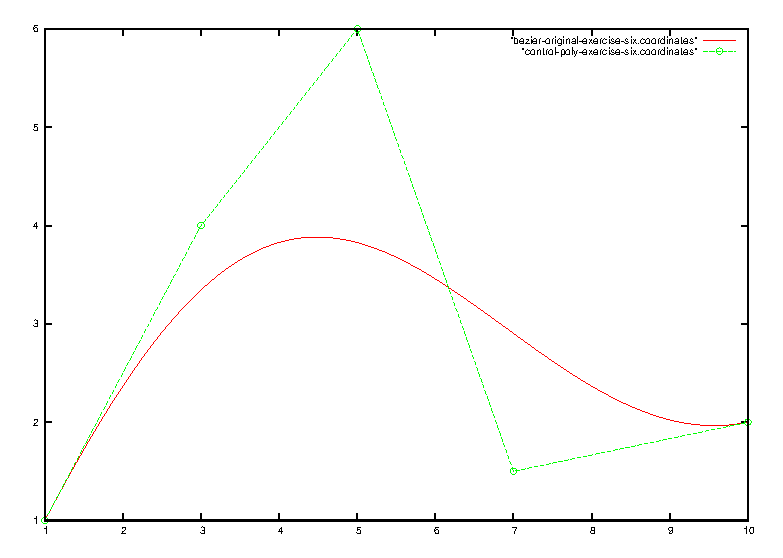
\includegraphics{bezier-deCasteljau-curves/exercise-six-original}
  \caption{Original curve before increasing degree}
  \label{fig:increasing-degree-original-curve}
\end{figure}
\begin{figure}
  \centering
  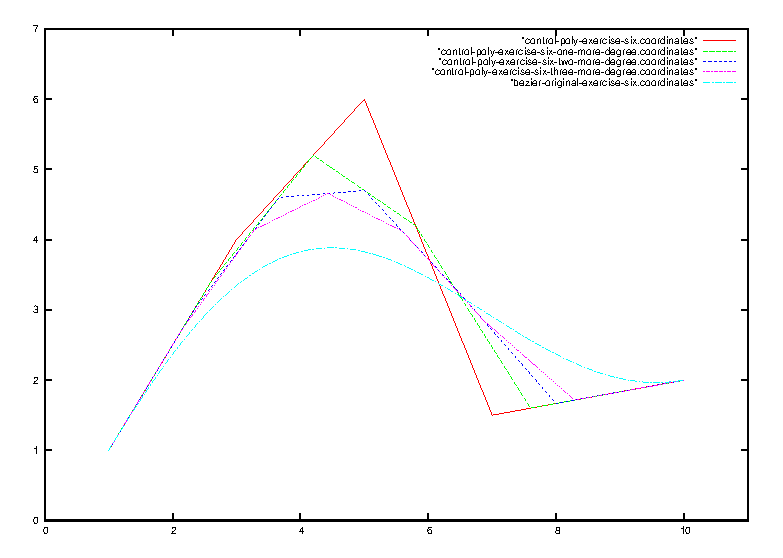
\includegraphics{bezier-deCasteljau-curves/exercise-six-higher-degree-control-poly}
  \caption{Some control polygons, each one with one more degree}
  \label{fig:some-increased-degrees}
\end{figure}
\begin{figure}
  \centering
  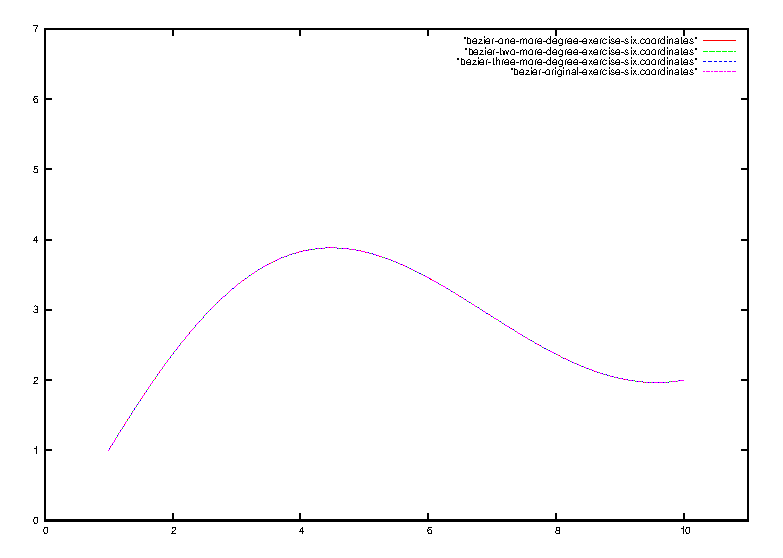
\includegraphics{bezier-deCasteljau-curves/exercise-six-one-more-degree-comparison}
  \caption{Increasing degree doesn't change the Bezier shape}
  \label{fig:increasing-degree-does-change-curve}
\end{figure}



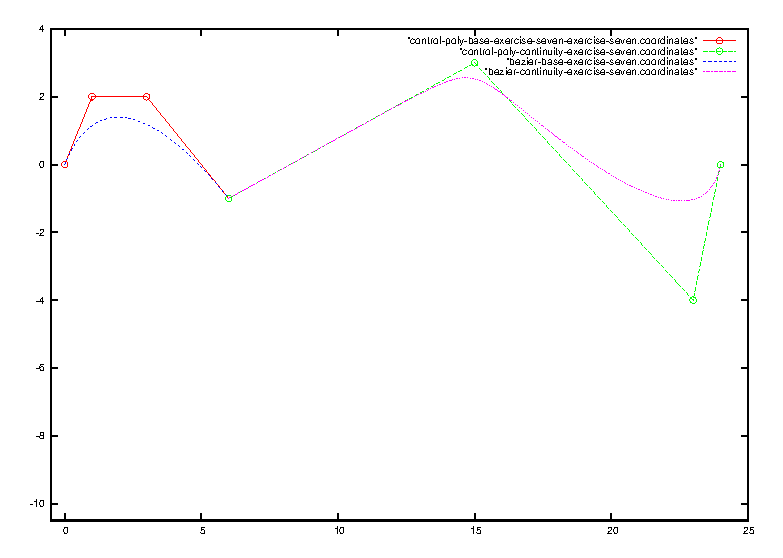
\includegraphics{bezier-deCasteljau-curves/exercise-seven-continuity}
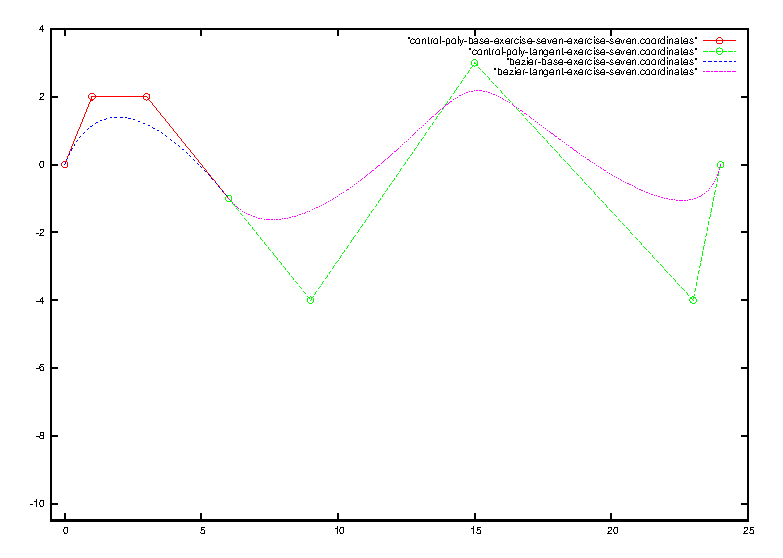
\includegraphics{bezier-deCasteljau-curves/exercise-seven-tangent}
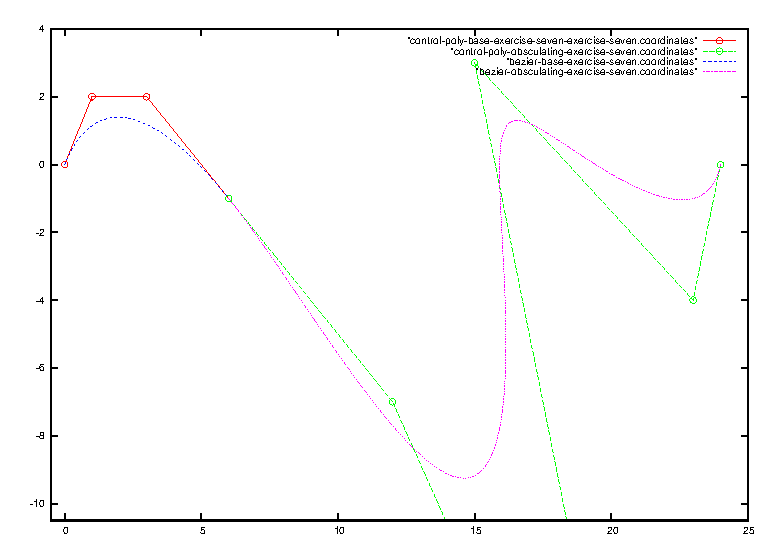
\includegraphics{bezier-deCasteljau-curves/exercise-seven-obsculating}
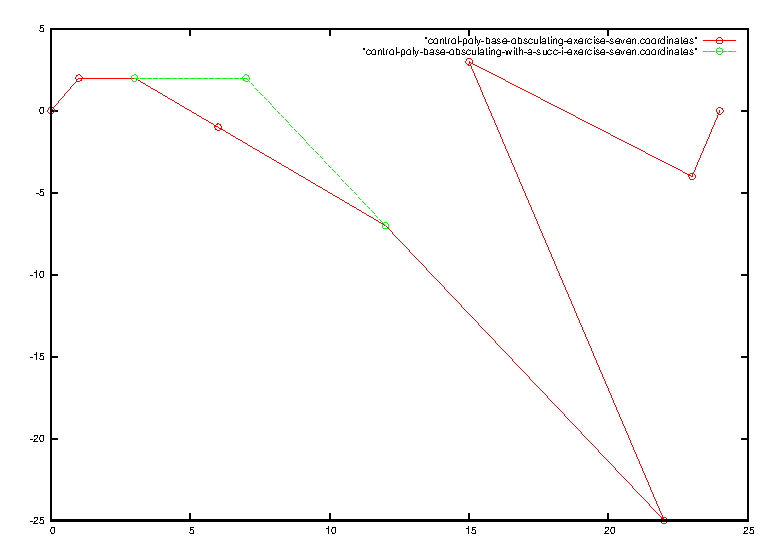
\includegraphics{bezier-deCasteljau-curves/exercise-seven-a_succ_i}
\includegraphics{bezier-deCasteljau-curves/exercise-seven-continuity-left}
\includegraphics{bezier-deCasteljau-curves/exercise-seven-tangent-left}
\includegraphics{bezier-deCasteljau-curves/exercise-seven-obsculating-left}
\includegraphics{bezier-deCasteljau-curves/exercise-seven-a_i-left}

\section{B-Splines}

\subsection{Mushrooms from clumped, uniformed and closed partitions}
\begin{figure}
  \centering
  \includegraphics{b-splines/exercise-zero-clumped.eps}
  \caption{Mushroom from clumped partition}
  \label{fig:clumpled-mushroom}
\end{figure}

\begin{figure}
  \centering
  \includegraphics{b-splines/exercise-zero-uniformed.eps}
  \caption{Mushroom from uniformed partition}
  \label{fig:uniformed-mushroom}
\end{figure}

\begin{figure}
  \centering
  \includegraphics{b-splines/exercise-zero-closed.eps}
  \caption{Mushroom from closed partition}
  \label{fig:closed-mushroom}
\end{figure}

\subsection{Increasing order $k$ while decreasing \emph{continuity} vector }
\begin{figure}
  \centering
  \includegraphics{b-splines/exercise-one-clumped.eps}
  \caption{Decreasing the \emph{continuity} vector collapsing in a Bezier }
  \label{fig:bspline-exercise-one-clumped}
\end{figure}

\subsection{Knots' multiplicities against the same control polygon}
\begin{figure}
  \centering
  \includegraphics{b-splines/exercise-two.eps}
  \caption{Knots's multiplicities increased against the same control polygon }
  \label{fig:bspline-exercise-two}
\end{figure}

\subsection{Linearity near doubled control point with a clumped partition}
\begin{figure}
  \centering
  \includegraphics{b-splines/exercise-three.eps}
  \caption{Linearity toward $(1,1)$ due to ``linearized'' convex hull}
  \label{fig:bspline-exercise-three}
\end{figure}

\subsection{Two clumped partitions, different \emph{continuity} vectors and same control polygon}
\begin{figure}
  \centering
  \includegraphics{b-splines/exercise-four.eps}
  \caption{Same control polygon with doubled $(0,6)$ againts two clumped partitions}
  \label{fig:bspline-exercise-four}
\end{figure}

\subsection{Increasing clumped partitions for increasing occurrences of a control point}
\begin{figure}
  \centering
  \includegraphics{b-splines/exercise-five.eps}
  \caption{Three B-Splines, each for $1,2,3$ occurrences of $(0,1)$ respectively }
  \label{fig:bspline-exercise-five}
\end{figure}

\subsection{Two B-Splines from two closed partitions}
\begin{figure}
  \centering
  \includegraphics{b-splines/exercise-six-first-closed.eps}
  \caption{A first B-Spline from a closed partition }
  \label{fig:bspline-exercise-six-first}
\end{figure}

\begin{figure}
  \centering
  \includegraphics{b-splines/exercise-six-second-closed.eps}
  \caption{A second B-Spline from a closed partition }
  \label{fig:bspline-exercise-six-second}
\end{figure}


\section{Code}

\subsection{de Casteljau}
\label{sec:deCasteljau-code}
\verbatiminput{bezier-deCasteljau-curves/deCasteljau.jl}

\subsection{Cox and de Boor}
\label{sec:Cox-deBoor-code}
\verbatiminput{b-splines/bspline.jl}

\newpage

\begin{thebibliography}{}

\bibitem{Julia} Open Source Project,
  \emph{Julia language}, \url{http://julialang.org/}

\bibitem{ETH} Locher T., Y. A. Pignolet, R. Wattenhofer,
  \textit{Principles of Distribuited Computing}, Zurich, Swiss Federal
  Institute of Technology, 2013.


\end{thebibliography}



\end{document}
